\section{Results}
\label{sec:results}

We tested our model using the following metrics: epoch loss, pixel accuracy, IoU score, and dice score.

\begin{table}[htbp]
    \centering
    \caption{Performance metrics}
    \label{tab:example}

    \begin{tabular}{|c|c|c|}
        \hline
        \textbf{} & \textbf{Background} & \textbf{Muscle layer} \\
        \hline
        \textbf{Pixel accuracy} & 0.1875 & 0 \\
        \textbf{IoU score} & 0.45 & 0 \\
        \textbf{Dice score} & 0.00285 & 0 \\
        \hline
    \end{tabular}

    \begin{tabular}{|c|c|c|}
        \hline
        \textbf{} & \textbf{Mucosal layer} & \textbf{Electrode} \\
        \hline
        \textbf{Pixel accuracy} & 0 & 0 \\
        \textbf{IoU score} & 0 & 0 \\
        \textbf{Dice score} & 0 & 0 \\
        \hline
    \end{tabular}

\end{table}

\begin{figure}[!]
    \centering
    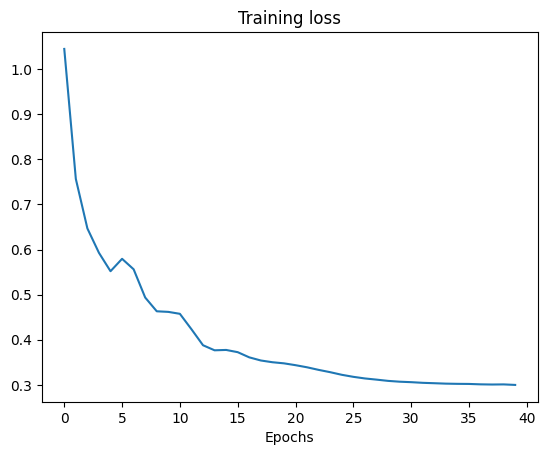
\includegraphics[width=0.4\textwidth]{Images/loss}
    \caption{Epoch loss}
    \label{fig:loss}
\end{figure}

\begin{figure}[htp!]
    \centering
    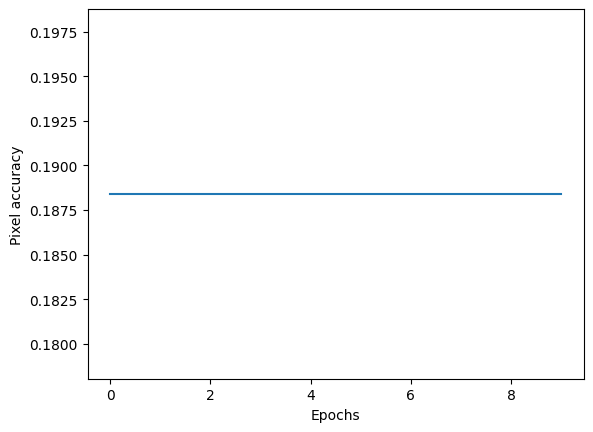
\includegraphics[width=0.4\textwidth]{Images/accuracy}
    \caption{Pixel accuracy}
    \label{fig:accuracy}
\end{figure}

\begin{figure}[htp!]
    \centering
    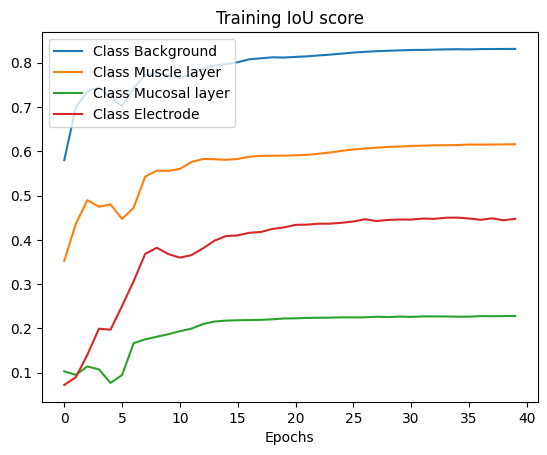
\includegraphics[width=0.4\textwidth]{Images/iou}
    \caption{IoU score}
    \label{fig:iou}
\end{figure}

\begin{figure}[!]
    \centering
    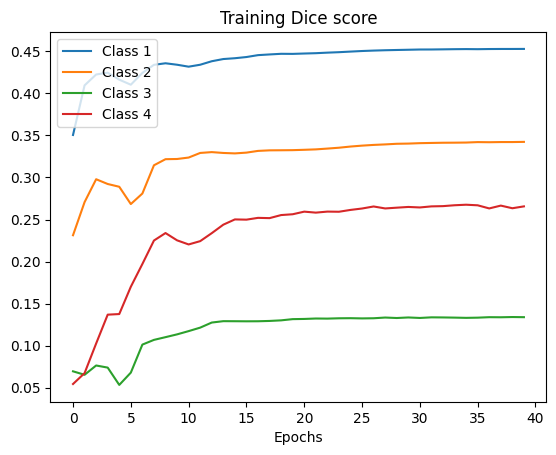
\includegraphics[width=0.4\textwidth]{Images/dice}
    \caption{Dice score}
    \label{fig:dice}
\end{figure}
